\documentclass[a4paper]{article}
\usepackage[utf8]{inputenc}
\usepackage{amsmath}
\usepackage{amsfonts}
\usepackage{amssymb}
\usepackage{graphicx}
\usepackage{geometry}
\usepackage[english]{babel}
\usepackage{enumitem}%can be used for automatic numbering of requirements/tests.
\usepackage{hyperref}
\usepackage[colorinlistoftodos]{todonotes}
\usepackage{color} % Used to write in red,blue,green etc.
\usepackage{float}
\usepackage[titletoc]{appendix}

\title{PUSS154253}
\newcommand{\version}{v 1.0}

\newcommand{\SVVS}{PUSS154213}

\author{Testgroup, Team 2}


%-------------------------TITLE-----------------------------------------

\begin{document}
\begin{titlepage}
\newgeometry{left=2cm,top=1cm,right=2cm}
\newcommand{\HRule}{\rule{\linewidth}{0.5mm}}

\begin{minipage}{0.5\textwidth}
\begin{flushleft} % Responsible persons, write on separate lines
\textit{Responsible for this document:}\\
Oskar Fällström %Not entirely sure who this should be, possibly project leaders as well?
\end{flushleft}
\end{minipage}
~
\begin{minipage}{0.4\textwidth}
\begin{flushright}
\title  %Dokumentnummer enl. projekthandledning s. 22-23 och insidan av pärmen
\today
\end{flushright}
\end{minipage}\\[3cm]

\centering
\textsc{\LARGE Team 2}\\[0.5cm]

\HRule \\[0.4cm]
{ \huge \bfseries Test Matrices for \SVVS\ v1.0 }\\[0.4cm] % Title of your document
\HRule \\[1.5cm]

\vfill
\begin{flushleft}
\textit{Authors of this document:}\\
Måns Andersson \\
Hanna Autio \\
Moa Eklöf \\
Oskar Fällström \\
Ulf Hörndahl \\
Jonathan Lundholm
\end{flushleft}


\end{titlepage}
\pagenumbering{gobble}

\begin{center}
\textit{\large Version History}

    \begin{tabular}{ | l | l | l | p{5cm} |}
    \hline
    \textbf{Version} 	& \textbf{Date} 	& \textbf{Responsible} 	& \textbf{Description} 		\\ \hline
    1.0				 	& 150915 			& UH 					&  Baseline. 				\\ \hline
    \end{tabular}
\end{center}

\newpage
%\pagenumbering{arabic}

\section{Test Matrices}
\begin{figure}[H]
    \centering
    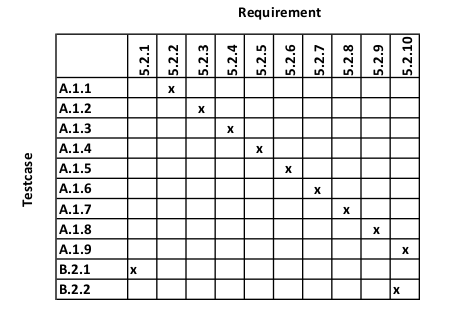
\includegraphics[scale=0.9]{SVVS-pics/testmatrixMyDevices.png}
    \caption{Test matrix for The My Devices View.}
    \label{fig:testmatrix-mydevices}
\end{figure}

\begin{figure}[H]
    \centering
    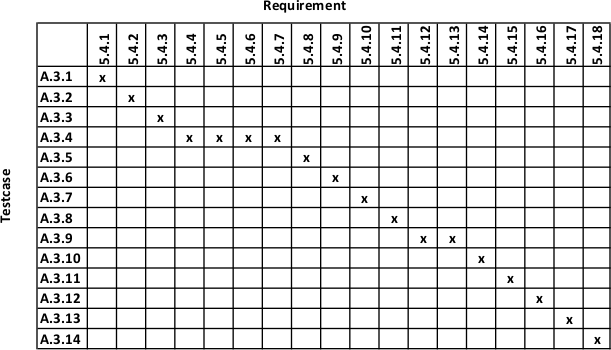
\includegraphics[scale=0.9]{SVVS-pics/testmatrixLightbulb.png}
    \caption{Test matrix for The Lightbulb View.}
    \label{fig:testmatrix-lightbulb}
\end{figure}

\begin{figure}[H]
    \centering
    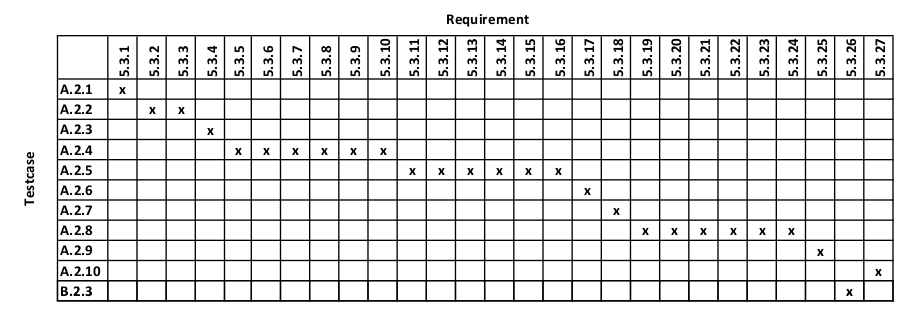
\includegraphics[scale=0.9,angle=-90]{SVVS-pics/testmatrixSensor.png}
    \caption{Test matrix for The Sensor View.}
    \label{fig:testmatrix-sensor}
\end{figure}

\begin{figure}[H]
    \centering
    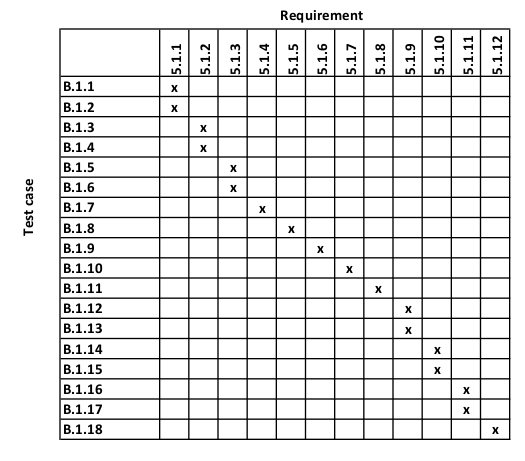
\includegraphics[scale=0.9]{SVVS-pics/testmatrixUsecases.png}
    \caption{Test matrix for the use cases.}
    \label{fig:testmatrix-usecase}
\end{figure}

\begin{figure}[H]
    \centering
    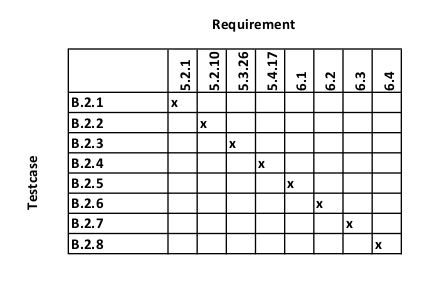
\includegraphics[scale=0.9]{SVVS-pics/testmatrixLayout.png}
    \caption{Test matrix for the layout.}
    \label{fig:testmatrix-layout}
\end{figure}

\end{document}